\documentclass[svgnames,14pt]{beamer}
\usepackage{caption}
\usepackage{graphicx}
\usepackage{xcolor}
\usepackage{wrapfig}
\usepackage{algorithm}
\usepackage{algpseudocode}
\title{Genomes Comparision via de Bruijn graphs}
\author{Student: Ilya Minkin \\ Advisor: Son Pham}
\institute{St. Petersburg Academic University}
\date{June 4, 2012}
\algnotext{EndFor}
\algnotext{EndIf}
\algnotext{EndWhile}
\setbeamertemplate{footline}[frame number]
\setbeamertemplate{navigation symbols}{}
\setbeamertemplate{caption}[numbered]
\begin{document}
\def\braces#1{[#1]}
\newenvironment{changemargin}[2]{% 
  \begin{list}{}{% 
    \setlength{\topsep}{0pt}% 
    \setlength{\leftmargin}{#1}% 
    \setlength{\rightmargin}{#2}% 
    \setlength{\listparindent}{\parindent}% 
    \setlength{\itemindent}{\parindent}% 
    \setlength{\parsep}{\parskip}% 
  }% 
  \item[]}{\end{list}}
\date{August 31, 2012}
\maketitle

\begin{frame}
\frametitle{Synteny Blocks: Algorithmic challenge}
\begin{itemize}
\item Suppose that we are given two genomes
\item The question is: how are they evolutionary related to each other?
\item In order to do rearrangements analysis we must decompose genomes into synteny blocks
\item Synteny blocks are evolutionary conserved segments of the genome
\item These blocks cover most of the genome
\item Occur in both genomes with possible variations
\end{itemize}
\end{frame}

\begin{frame}
\frametitle{Academic Project}
Project: Identify synteny blocks for duplicated genomes represented as sequences of \textbf{nucleotides}.
\begin{itemize}
\item \textbf{None} of the previous synteny blocks reconstruction software (DRIMM-Synteny (Pham and Pevzner 2010) included) can 
efficiently solve this problem. 
\item DRIMM-Synteny can find the synteny blocks for complicated genomes. But:
\pause \item It requires the genome to be represented as sequence of genes. 
\end{itemize}
\end{frame}

\begin{frame}
\frametitle{General Idea: de Bruijn Graph}
\begin{itemize}
\item We are given an alphabet \( \Sigma \) and a string \( S \) over it, \(|\Sigma| = m \)
\item A substring \( T, \, |T| = k \) is called \textit{k-mer}
\item De Bruijn graph is a multigraph \( G_{k} = (V, E) \), where \\
\( V = \Sigma^{k - 1} = \) \{all possible \( (k - 1) \)-mers\} \\
\item If \(k\)-mer \( T \) is presented in \( S \), then we add an oriented edge \( (T[1, k - 1], T[2, k]) \) to the graph
\item Create de Bruijn graph from the nucleotide sequence
\item Conserved regions will yield non-branching paths
\end{itemize}
\end{frame}

\begin{frame}
\frametitle{Challenges}
\begin{itemize}
\item Variations in synteny blocks generate cycles, so we need to simplify the graph
\item Double strandness: conserved regions may occur on both strands. Example: \\
5' \textcolor{Green}{AACC}GGTT 3' \\
3' TTGG\textcolor{Green}{CCAA} 5' \\
Such blocks are reverse complementary to each other \( \Rightarrow \) no non-branching paths
\item We need exact shared \(k\)-mers, so \textit{directly} our approach can be applied
to closely related species (different strains of a bacteria, etc)
\item Efficiency
\end{itemize}
\end{frame}

\begin{frame}
\frametitle{Colored graph}
\begin{itemize}
\item We use colored de Bruijn graphs \\
\braces{Iqball et al., 2012} to handle double-strandness
\item Suppose that \( S^{+} \) and \( S^{-} \) are positive and negative strands of the chromosome
\item Colored de Bruijn graph  is a multigraph \( G_{k} = (V, E) \) where \( V =  \Sigma^{k - 1} \)
\item For each \(k\)-mer \(T^{+}\) in \(S^{+}\) add edge \( (T^{+}[1, k - 1], T^{+}[2, k]) \) to \( G_{k} \) and mark it \\ \textit{blue}
\item For each \(k\)-mer \(T^{-}\) in \(S^{-}\) add edge \( (T^{-}[1, k - 1], T^{-}[2, k]) \) to \( G_{k} \) and mark it \\ \textit{red}
\end{itemize}
\end{frame}

\begin{frame}
\frametitle{Edge labeling}
\begin{itemize}
\item Note that our graph is built from a string, not set of reads
\item Each walk in the graph represents a string
\item We are interested only in walks that represent substrings of the source string
\item Assign to each edge \( e \) label \( L(e) = \) position of the corresponding  \(k\)-mer on the positive strand
\item Walk  \( W = ( v_{1} \, e_{1} \, v_{2} \, e_{2} \, ... ) \) is considered valid iff: \\
1. \( e_{i} \) and \( e_{i + 1} \) are of the same color \\
2. \( | L(e_{i}) - L(e_{i + 1}) | = 1 \)
\end{itemize}
\end{frame}

\begin{frame}
\frametitle{Example}
\begin{changemargin}{-1.cm}{-1.cm}
\begin{figure}
\centering
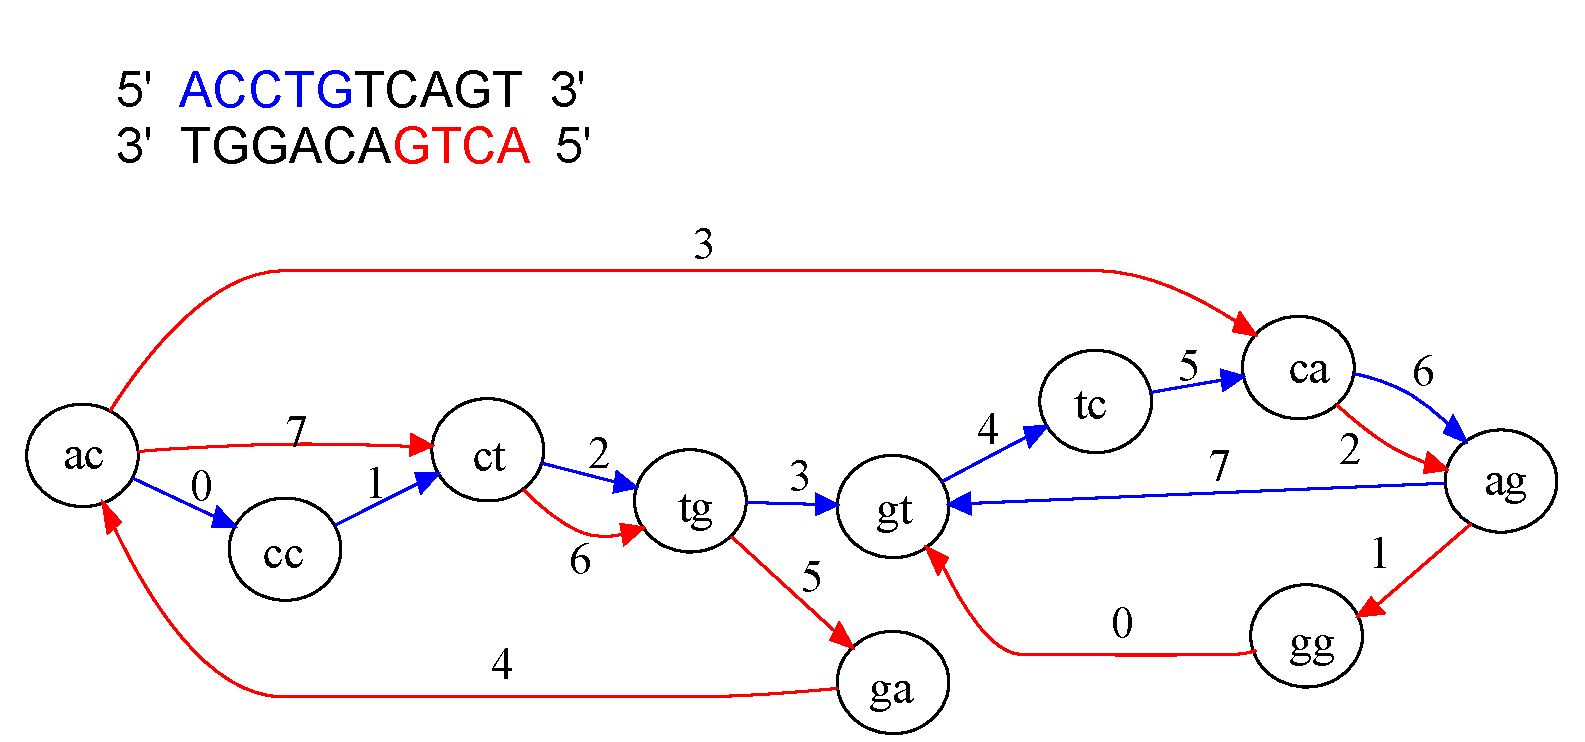
\includegraphics[scale = 0.480]{Figure1.pdf}
\small \caption{Colored de Bruijn graph built from two strands}
\end{figure}
\end{changemargin}
\end{frame}

\begin{frame}
\frametitle{Graph simplification}
\begin{itemize}
\item Bulges spoil long non-branching paths and indicate indels/mismatches
\item A pair of walks \((W_{1}, W_{2})\) is a bulge iff: \\
1) Start and end vertices of  \(W_{1} \) and  \(W_{2}\) coincide\\
2) \(W_{1} \) and  \(W_{2}\) have exactly 2 common vertices \\
3) There are no edges \(u \in W_{1} \) and \( v \in W_{2}\) such that \(L(u) = L(v) \) \\
4) \(|W_{1}|  \leq \delta \) and \(|W_{2}| \leq \delta \)
\end{itemize}
\begin{changemargin}{-1.cm}{-1.cm}
\begin{figure}
\centering
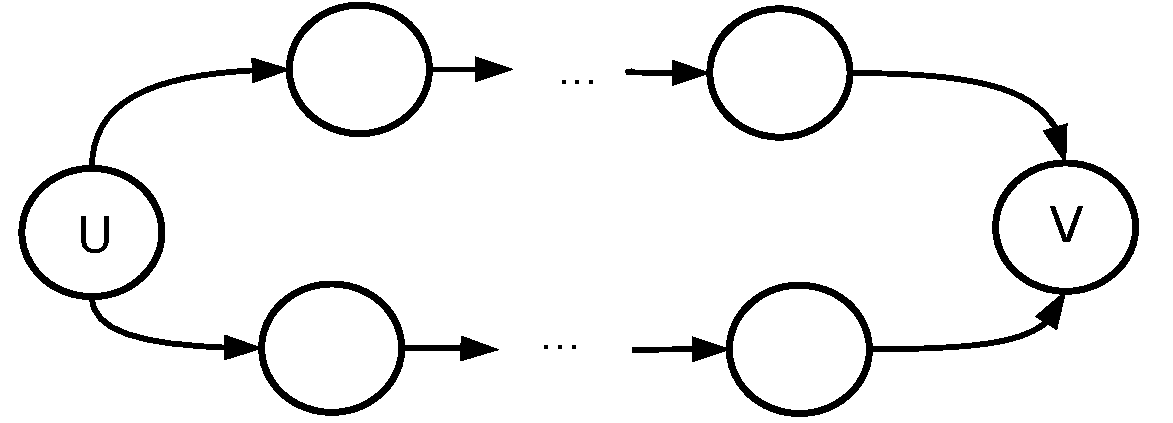
\includegraphics[scale = 0.30]{Figure2.pdf}
\small \caption{A bulge}
\end{figure}
\end{changemargin}
\end{frame}

\begin{frame}
\frametitle{General pipeline}
\begin{itemize}
\item Build de Bruijn graph from the genome
\item Remove bulges
\item Bulges are removed by replacing one branch with another
\item Output non-branching paths
\end{itemize}
\begin{changemargin}{-1.cm}{-1.cm}
\begin{figure}
\centering
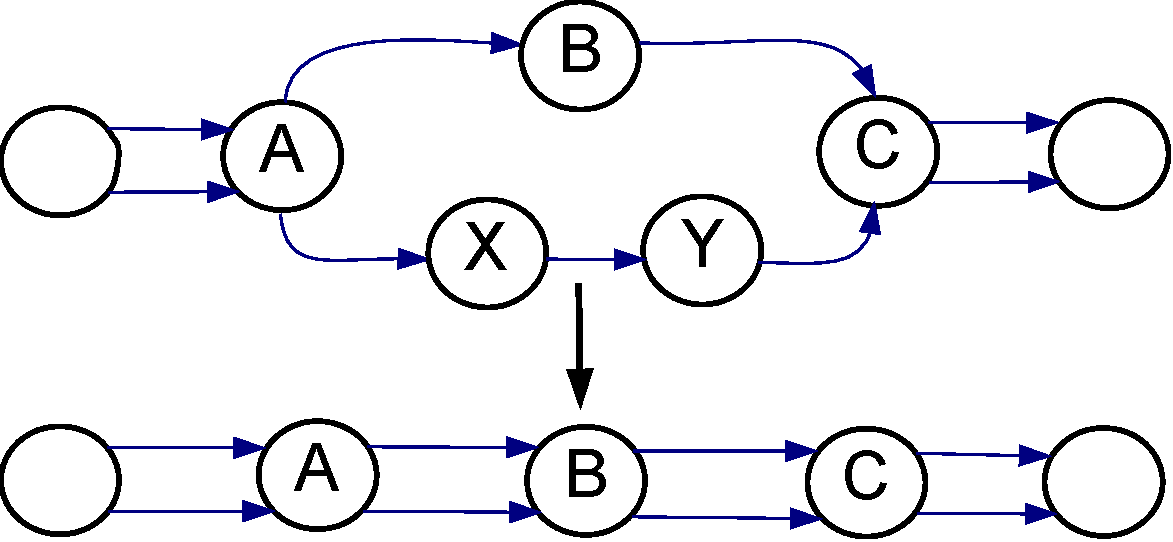
\includegraphics[scale = 0.45]{Figure3.pdf}
\small \caption{Bulge removal illustration}
\end{figure}
\end{changemargin}
\end{frame}

\begin{frame}
\frametitle{Bulge removal strategy}
\begin{itemize}
\item It does matter which bulge's branch we replace
\item Synteny blocks with muliplicity \(>2\) can have no \(k\)-mers shared across all instances of a same block
\item Example: a synteny block from yeasts \braces{Kellis et al., 2004}
\begin{changemargin}{-1.cm}{-1.cm}
\begin{figure}
\centering
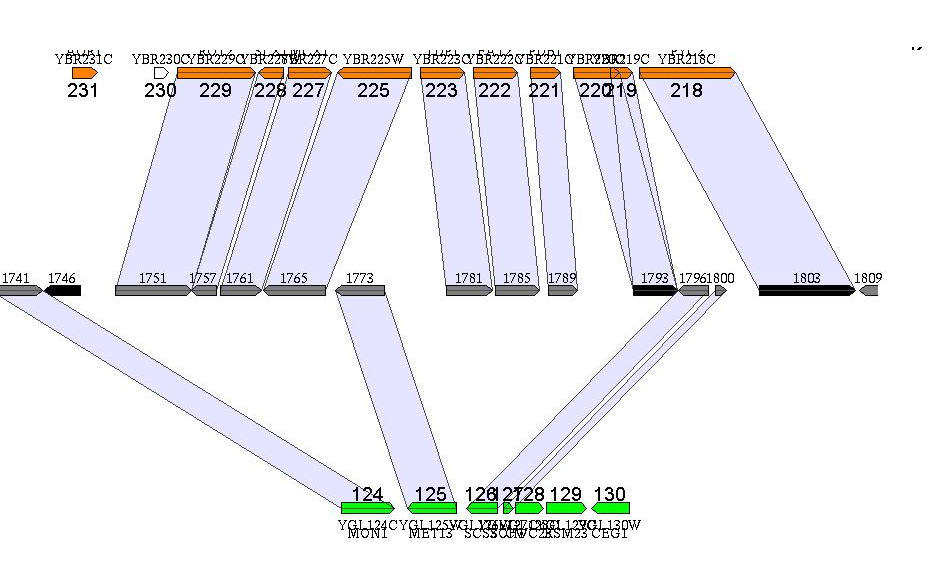
\includegraphics[scale = 0.30]{Figure5.png}
\small \caption{A synteny block example}
\end{figure}
\end{changemargin}
\end{itemize}
\end{frame}

\begin{frame}
\frametitle{Bulge removal strategy}
\begin{itemize}
\item Suppose that we have synteny 3 regions, \(k\)-mers are denoted by integers: \\
2 4 6 \\
1 2 3 4 5 6 \\
1 3 5 \\
\item Let's build de Bruijn graph for this situation:
\begin{changemargin}{-1.cm}{-1.cm}
\begin{figure}
\centering
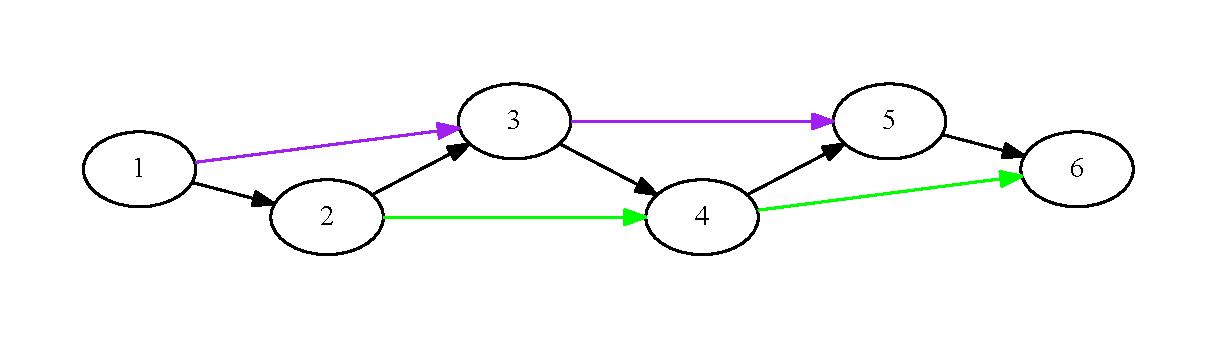
\includegraphics[scale = 0.50]{graph1.pdf}
\end{figure}
\end{changemargin}
\end{itemize}
\end{frame}

\begin{frame}
\frametitle{Wrong strategy}
\begin{itemize}
\item Initial situation:
\begin{changemargin}{-1.cm}{-1.cm}
\begin{figure}
\centering
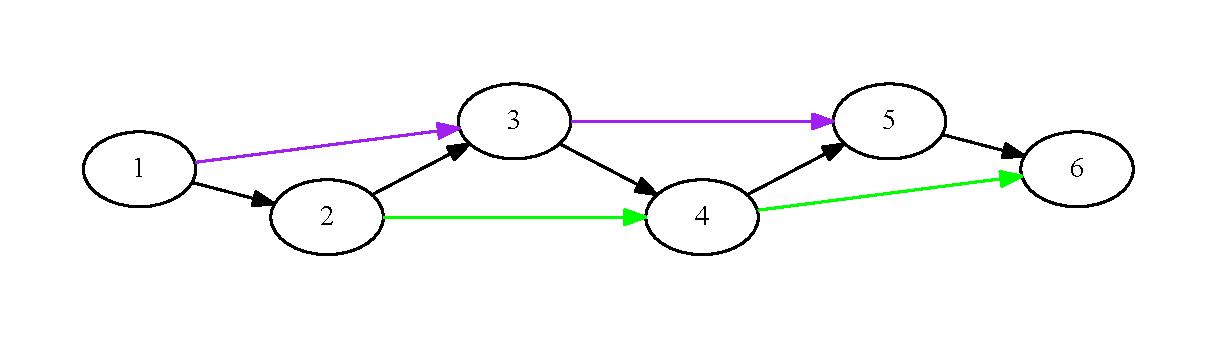
\includegraphics[scale = 0.38]{graph1.pdf}
\end{figure}
\end{changemargin}
\item Replace 1 3 by 1 2 3:
\begin{changemargin}{-1.cm}{-1.cm}
\begin{figure}
\centering
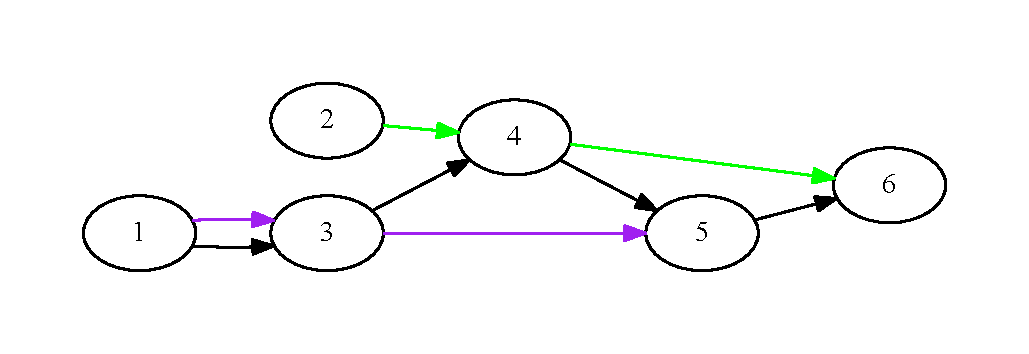
\includegraphics[scale = 0.38]{graph2.pdf}
\end{figure}
\end{changemargin}
\item Replace 3 4 5 by 3 5:
\begin{changemargin}{-1.cm}{-1.cm}
\begin{figure}
\centering
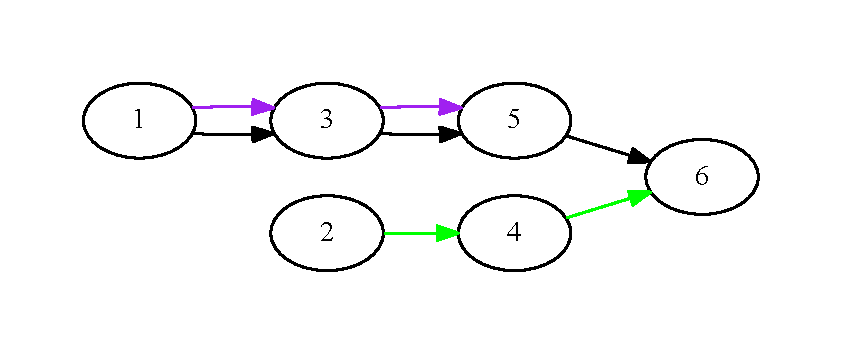
\includegraphics[scale = 0.38]{graph3.pdf}
\end{figure}
\end{changemargin}
\end{itemize}
\end{frame}

\begin{frame}
\frametitle{Proper strategy}
\begin{itemize}
\item Initial situation:
\begin{changemargin}{-1.cm}{-1.cm}
\begin{figure}
\centering
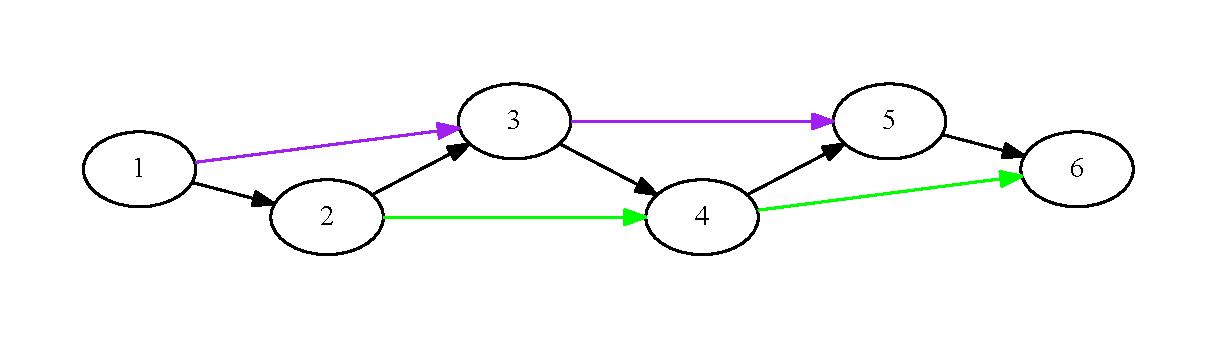
\includegraphics[scale = 0.38]{graph1.pdf}
\end{figure}
\end{changemargin}
\item Replace 1 3 by 1 2 3:
\begin{changemargin}{-1.cm}{-1.cm}
\begin{figure}
\centering
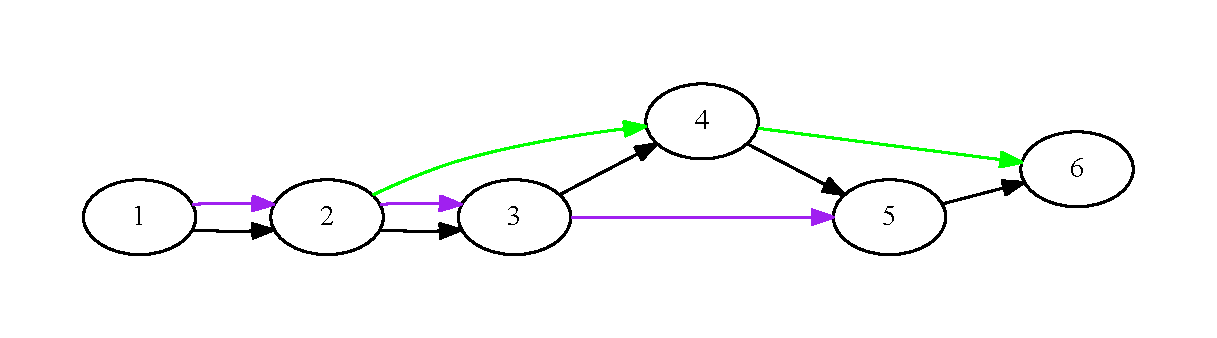
\includegraphics[scale = 0.38]{graph4.pdf}
\end{figure}
\end{changemargin}
\item Replace 4 6 by 4 5 6:
\begin{changemargin}{-1.cm}{-1.cm}
\begin{figure}
\centering
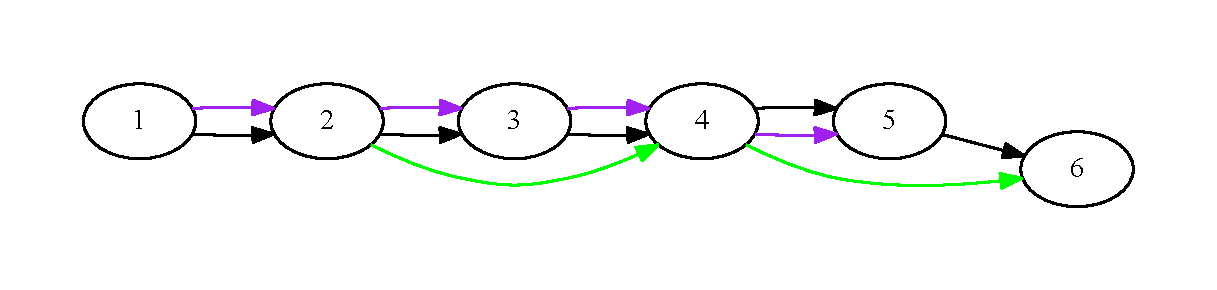
\includegraphics[scale = 0.38]{graph5.pdf}
\end{figure}
\end{changemargin}
\end{itemize}
\end{frame}

\begin{frame}
\frametitle{Proper strategy}
\begin{itemize}
\item From previous slide:
\begin{changemargin}{-1.cm}{-1.cm}
\begin{figure}
\centering
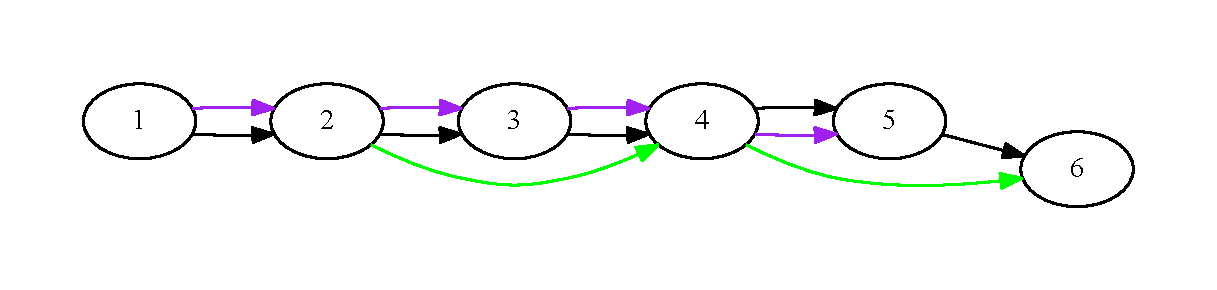
\includegraphics[scale = 0.38]{graph5.pdf}
\end{figure}
\end{changemargin}
\item Replace 2 4 by 2 3 4:
\begin{changemargin}{-1.cm}{-1.cm}
\begin{figure}
\centering
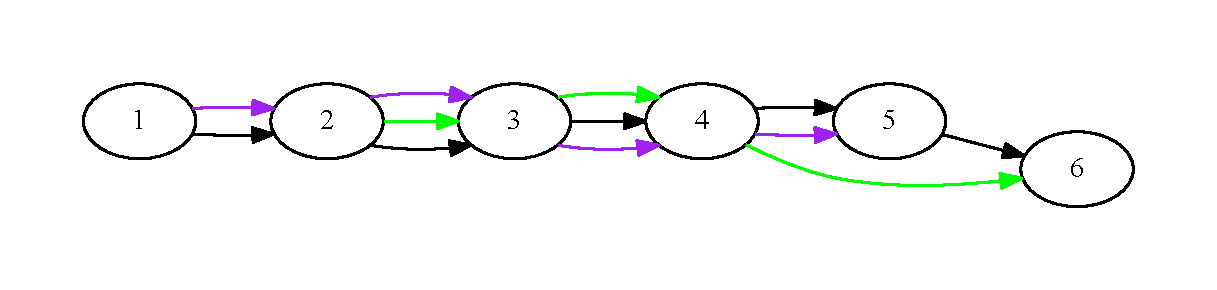
\includegraphics[scale = 0.38]{graph6.pdf}
\end{figure}
\end{changemargin}
\item Replace 4 5 by 4 5 6:
\begin{changemargin}{-1.cm}{-1.cm}
\begin{figure}
\centering
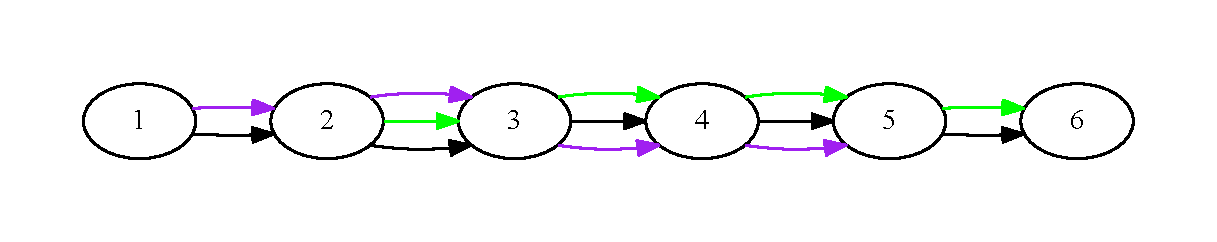
\includegraphics[scale = 0.38]{graph7.pdf}
\end{figure}
\end{changemargin}
\end{itemize}
\end{frame}

\begin{frame}
\frametitle{Proper strategy}
\begin{itemize}
\item We incapsulate this intuition into a heuristic
\item A vertex \(v\) in the graph is called \textit{bifurcation} if there are at least two ingoing (outgoing) edges incident \(v\) that spell different \(k\)-mers.
\item Let's denote by \(MaxBif(p)\) maximum degree of bifurcation that lies on path \(p\)
\item If two paths \(p_1\) and \(p_2\) form a bulge, then we replace \(p_1\) by \(p_2\) iff \(MaxBif(p_1) > MaxBif(p_2)\), otherwise we replace 
\(p_2\) by \(p_1\)
\item And it seems to work
\end{itemize}
\end{frame}

\begin{frame}
\frametitle{Results: a simple example}
\begin{itemize}
\item We took two bacteria from \textit{Pseudomonas aeruginosa} group and dot plot them: \\
\textit{Pseudomonas aeruginosa PAO1} \\
\textit{Pseudomonas aeruginosa UCBPP-PA14} \\
\begin{changemargin}{-1.cm}{-1.cm}
\begin{figure}
\centering
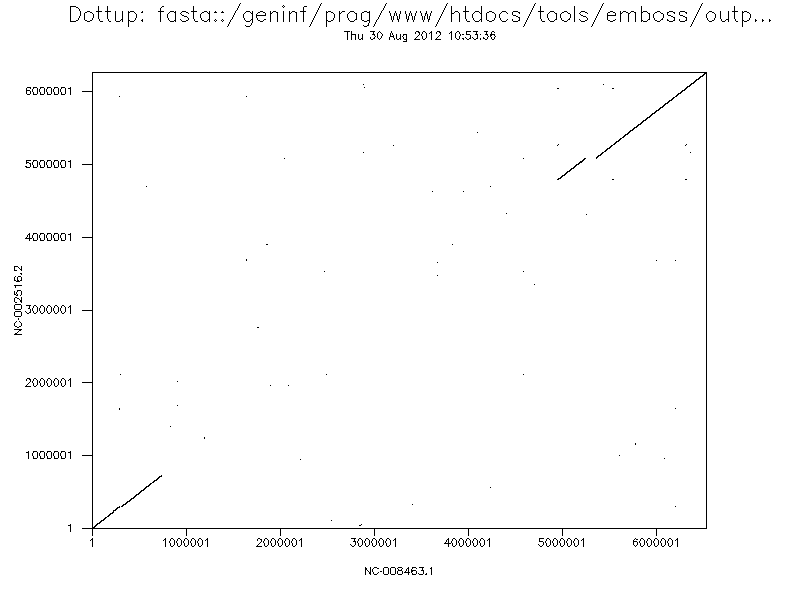
\includegraphics[scale = 0.20]{PA01POS_PA14POS.png}
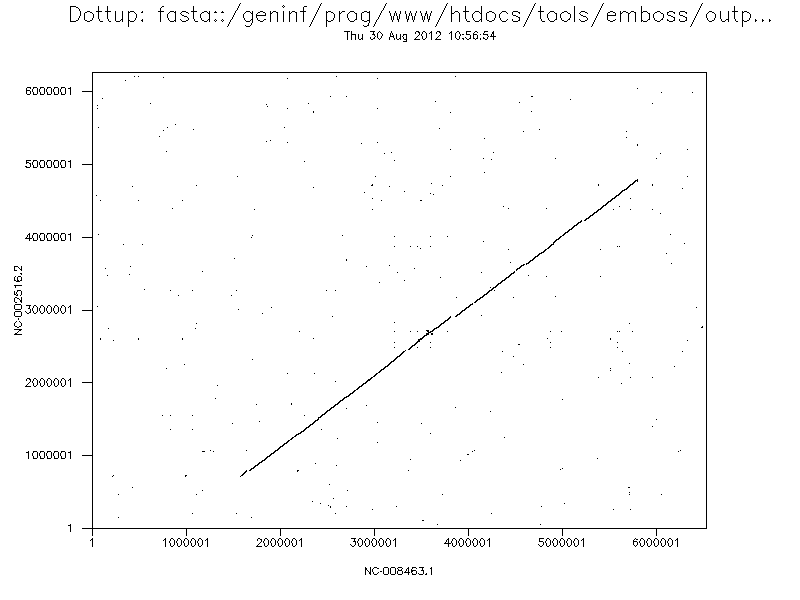
\includegraphics[scale = 0.20]{PA01NEG_PA14POS.png}
\small \caption{Left plot corresponds to PA01 against PA14, right plot corresponds to reverse-complementary of PA01 against PA14}
\end{figure}
\end{changemargin}
\end{itemize}
\end{frame}

\begin{frame}
\frametitle{Results: a simple example}
\begin{itemize}
\item Then we constructed the blocks using our program
\item \(K = 5000, \delta = 25000\)
\item Results: \\
+9 -0 -1 -2 -3 -4 -5 -6 +7 +10 +8 \\
+9 -7 +6 +5 +4 +3 +2 +1 +0 +10 +8 \\
\end{itemize}
\end{frame}

\begin{frame}
\frametitle{Results: three bacteria dataset}
\begin{itemize}
\item Three strains of \textit{Mycobacterium tuberculosis H37Rv}: \\
Laboratory reference strain \textit{H37Rv} \\
CCDC5180 \\
CCDC5079 \\
\item One of this strains has multiple drugs resistance
\item We use \(K = 1000\) and \(\delta = 5000\)
\item Blocks with multiplicity 3 cover 96\% of the genome
\item And Son see an evidence of rearrangements there
\end{itemize}
\end{frame}

\begin{frame}
\frametitle{Results: three bacteria dataset}
\begin{changemargin}{-1.cm}{-1.cm}
\begin{figure}
\centering
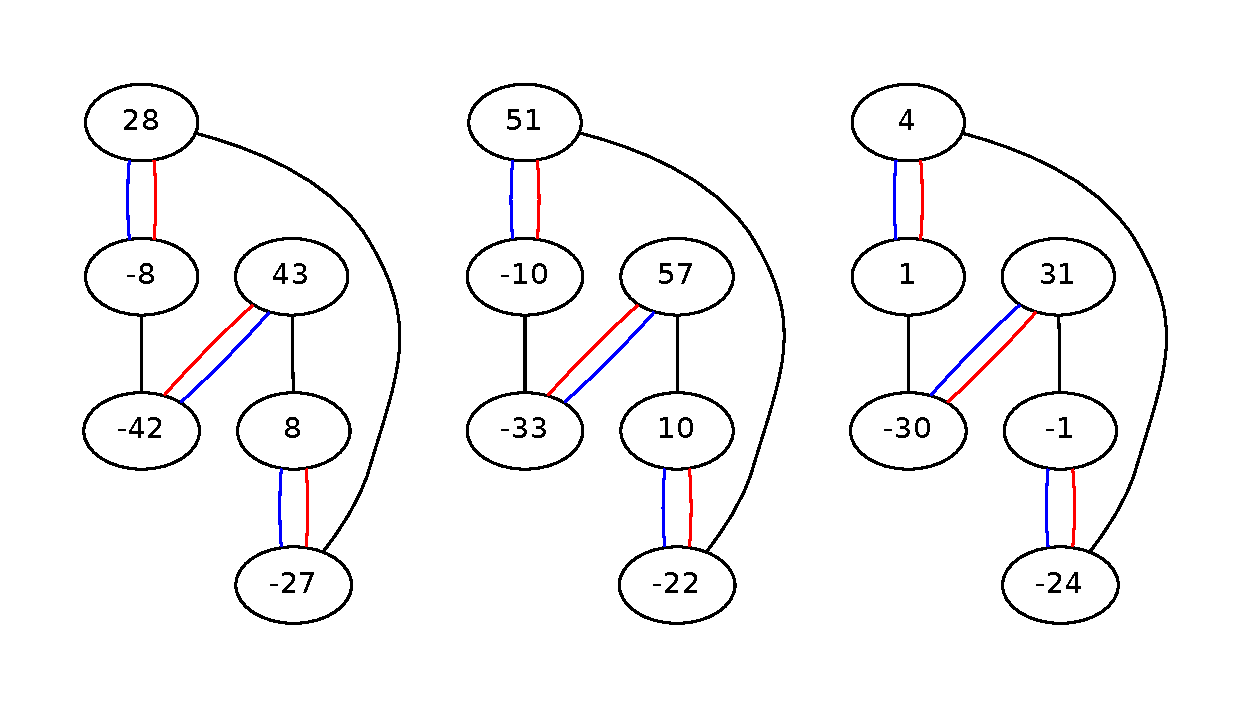
\includegraphics[scale = 0.50]{tuber.pdf}
\small \caption{}
\end{figure}
\end{changemargin}
\end{frame}

\begin{frame}
\frametitle{Results: yeasts dataset}
\begin{itemize}
\item Well known research about yeasts \textit{Saccharomyces cerevisiae} and \textit{Kluyveromyces waltii} \braces{Kellis et al., 2004} 
\item This paper shows evidence of so called \textit{double conserved synteny} regions: one region (block) in k.waltii corresponds to two
regions in cerevisiae
\item We can't apply our method directly. But we can use alignments of ORFs from 
the paper to enrich number of \(k\) mers
\item With \(k = 1000\) and \(\delta = 20 000 \) we cover 67\% of the genome by blocks with multiplicity 3. Our blocks match 212 blocks
from overall 252 in Kellis paper
\end{itemize}
\end{frame}

\begin{frame}
\frametitle{Conclusions}
\begin{itemize}
\item Our method is applicable for reconstructing synteny blocks in closely related species
\item It can be extendede to handle more complicated cases
\end{itemize}
Future plans:
\begin{itemize}
\item Perform additional tests and evaluations
\item Release software for finding synteny blocks in closely related species (end of Setptember)
\item Write a paper
\item Incorporate a local alignment tool and extend range of use to more complicated cases
\end{itemize}
\end{frame}

\begin{frame}
\frametitle{References}
\begin{itemize}
\item 1. Pevzner P and Tesler G, (2003) Human and mouse genomic sequences reveal extensive breakpoint reuse in mammalian evolution. 
\item 2. Pham S and Pevzner P, (2010) DRIMM-Synteny: Decomposing Genomes into Evolutionary Conserved Segments
\item 3. Iqbal Z, Caccamo M, Turner I, Flicek P, McVean G, (2012) De novo assembly and genotyping of variants using colored de Bruijn graphs
\item 4. Arabidopsis Genome Initiative, (2000) Analysis of the genome sequence of the flowering plant Arabidopsis thaliana
\item 5. Kellis M, W. Birren B, S. Lander E, (2004) Proof and evolutionary analysis of ancient genome duplication in the yeast Saccharomyces cerevisiae.
\end{itemize}
\end{frame}

\begin{center}
\hfill \huge \\
\vspace{60pt}
Thank you!
\end{center}

\end{document}
